%Preamble
%!TeX TXS-program:compile = txs:///pdflatex/[--shell-escape]
\documentclass[11pt,letterpaper,twocolumn]{article}
\usepackage[spanish,es-tabla]{babel} % idioma: Español, no coloque nombre tablas como cuadro
\usepackage[T1]{fontenc} \usepackage[utf8]{inputenc} % símbolos especiales del idioma
\usepackage{times}
\usepackage[calc,showdow,spanish]{datetime2}
%\parindent = 0cm % configuración de sangría
\usepackage[backend=biber,style=ieee]{biblatex}
\usepackage{tabularx} % extra features for tabular environment
%\usepackage{amsmath} \usepackage{amssymb,amsfonts,latexsym,cancel}  % símbolos matemáticos 
%\usepackage{array}
%\usepackage{bm}
%\usepackage{epstopdf} % figuras en formato eps a pdf
\usepackage{hyperref} % agregar hiper enlaces dentro del archivo PDF generado
%\usepackage{longtable} % habilitar tablas largas
%\setcounter{MaxMatrixCols}{40} % configuración de limite columnas: 40
%\usepackage{multicol} % varias columnas al documento
%\usepackage{subfigure} % varias figuras
\usepackage[small,compact]{titlesec} \usepackage{titling} %cambiar el formato del titulo
%\newcolumntype{E}{>{$}c<{$}} % información de tablas en formato matemático
\usepackage{graphicx} % takes care of graphic including machinery
\usepackage{geometry} % configuración del dimensiones de la margen del documento 
\usepackage{filecontents}
\usepackage{pgfplots} % graficas de funciones matematicas
\pgfplotsset{compat=newest}
\usepgfplotslibrary{fillbetween}
\usepackage{siunitx}
\usepackage{pgfplotstable}
\usepackage{booktabs}
\usepackage{xcolor}
% \usepackage{LobsterTwo}
\usepackage{subcaption}
\usepackage{svg} % insertar imagenes .svg
\usepackage{tcolorbox}
\usepackage{fancyhdr} % configuración del formato del documento
\usepackage{authblk}
\usepackage[font=footnotesize]{caption}
\usepackage[toc,page]{appendix}
\usepackage{parskip}
\usepackage{amssymb, amsmath} % Paquetes matemáticos de la American Mathematical Society
\usepackage{float}
\usepackage{setspace}
\usepackage{parskip}
\usepackage{multirow}
\usepackage[all]{xy}
\usepackage{pstricks-add}
\usepackage{tikz}
\usepackage{circuitikz}
\usetikzlibrary{positioning,circuits.ee.IEC}
\usetikzlibrary{matrix}
\usetikzlibrary{calc}
\usetikzlibrary{fit}
\usetikzlibrary{shapes.geometric}
%\usepackage{showframe}


% *********************************************************
% *********************************************************
% ************* CONFIGURACIÓN DE PAQUETS ****************** 
% *********************************************************
% *********************************************************
%---------------------------------------------
% configuración formato de fecha
\DTMnewdatestyle{mydateformat}{%
	\renewcommand{\DTMdisplaydate}[4]{%
		%\DTMshortweekdayname{##4},\space% short weekday,
		%\DTMmonthname{##2}\nobreakspace%  (full) Month
		%\number##3,\space%                day,
		%\number##1%                       year
	}%
	\renewcommand{\DTMDisplaydate}{\DTMdisplaydate}%
}
%---------------------------------------------
% configuración de margen
\geometry{
	papersize = {216mm, 279.4mm},
	width = 20cm,
	height = 25cm,
	headsep = 5mm,
	head = 2cm,
	marginpar = 2mm,
	includeall,
}
%---------------------------------------------
% configuración de hiper vínculos
\hypersetup{
	colorlinks=true,       % false: boxed links; true: colored links
	linkcolor=black,        % color of internal links
	citecolor=black,        % color of links to bibliography
	filecolor=magenta,     % color of file links
	urlcolor=black
}
%---------------------------------------------
% configuración de estilo de la margen
\fancyhf{}
\renewcommand{\headrulewidth}{0pt}
\fancyhead[LO,L]{
	
\includegraphics[scale=0.119]{img/escudo.jpg}
}
\fancyhead[RO,R]{
	\fontsize{9}{9}
	\textsf{
		Modulación y demulación a una señal\\
		Teoría de telecomunicaciones I, Grupo A12\\
		\vspace{-1.3mm}
		\today
		\DTMsetdatestyle{mydateformat}
		\today
	}
}
\fancyfoot[C]{\thepage}
\pagestyle{fancy}
%---------------------------------------------
\spanishdecimal{.}
\tcbuselibrary{theorems}
%---------------------------------------------
% configuración para sección de archivos e información adicional al documento
\addto\captionsspanish{
	\renewcommand\appendixname{Anexo}
	\renewcommand\appendixpagename{Anexos}
}
%---------------------------------------------
% algunas configuraciones del cuerpo del documento
\renewcommand{\tablename}{Tabla}
\renewcommand{\baselinestretch}{0.8} % Para indicar el tamaño del entrelineado
\titleformat{\subsection}[wrap]
{\large\normalfont\fontseries{b}\selectfont\filright}
{\thesubsection.}{.5em}{}
\titlespacing{\subsection}
{12pc}{1.5ex plus .1ex minus .2ex}{1pc}

\titleformat{\section}[wrap]
{\large\normalfont\fontseries{b}\selectfont\filright}
{\thesection.}{.5em}{}
\titlespacing{\section}
{12pc}{1.5ex plus .1ex minus .2ex}{1pc}
\setlength{\parskip}{1.5mm} % Modificar espacio entre párrafos
\renewcommand*{\bibfont}{\footnotesize} % Cambiar tamaño bibliografía
%---------------------------------------------
% configuración de estilo para autores y afiliaciones
\renewcommand*{\Authsep}{ y }
\renewcommand*{\Authand}{ y }
\renewcommand*{\Authands}{, }
\renewcommand*{\Affilfont}{\normalsize}
%\renewcommand*{\Authfont}{\bfseries}    % make author names boldface    
\setlength{\affilsep}{-2mm}   % set the space between author and affiliation
\renewcommand\Authfont{\fontsize{12}{12}\selectfont} % Cambiar tamaño de letra autores
\renewcommand\Affilfont{\fontsize{9}{9}\itshape} % Cambiar tamaño de letra afiliaciones de autores
%---------------------------------------------
% Simbolo fuente AC
\tikzset{circuit declare symbol = ac source}
\tikzset{set ac source graphic = ac source IEC graphic}
\tikzset{
	ac source IEC graphic/.style={
			transform shape,
			circuit symbol lines,
			circuit symbol size = width 3 height 3,
			shape=generic circle IEC,
			/pgf/generic circle IEC/before background={
					\pgfpathmoveto{\pgfpoint{-0.8pt}{0pt}}
					\pgfpathsine{\pgfpoint{0.4pt}{0.4pt}}
					\pgfpathcosine{\pgfpoint{0.4pt}{-0.4pt}}
					\pgfpathsine{\pgfpoint{0.4pt}{-0.4pt}}
					\pgfpathcosine{\pgfpoint{0.4pt}{0.4pt}}
					\pgfusepathqstroke
				}
		}
}
%---------------------------------------------

%\brokenpenalty=10000 
%\hyphenpenalty=5000 
\raggedbottom
%---------------------------------------------
% Titulo, autores e información afiliada a los autores
\title{
	\fontsize{22}{22}\selectfont
	\vspace{-9mm}
	\textbf{Modulaciones Lineales
		\vspace{-1mm}}}
\author[1]{Jefry Nicolás Chicaiza}
\author[2]{Jose Nicolás Zambrano}
\affil[1]{\url{jefryn@unicauca.edu.co}
	\vspace{-2mm}}
\affil[2]{\url{jnzambranob@unicauca.edu.co}
	\vspace{-5mm}}
\date{}
%---------------------------------------------
% vincular archivo de bibliografías
\bibliography{codigofuente/bibliografia}
%---------------------------------------------
% cuerpo del documento
\begin{document}
%---------------------------------------------
% retornar configuraciones realizadas en preámbulo al cuerpo del documento
\maketitle
\thispagestyle{fancy}
%---------------------------------------------
\section{Introducción}%
\label{sec:introduccion}

El informe del Trabajo 5 de la asignatura Teoría de las Telecomunicaciones 1 se desarrolla en este documento. El trabajo consiste en considerar una señal planteada de tipo diente de sierra no periódica para aplicar los teoremas de modulaciones lineales.

Iniciar con el desarrollo analítico es necesario debido a que para alcanzar los resultados esperados en la simulación, se requiere conocer de antemano los efectos que representa al aplicar los conceptos de Modulaciones Lineales a la señal, esto permitirá comprobar los resultados obtenidos por medio de un algoritmo realizado en MATLAB.

El objetivo de dicha simulación al aplicar los conceptos del tema es realizar una modulación y demodulación de la señal a partir de la Modulación de Doble Banda Lateral con Portadora Suprimida(DSBSC), el cual es un esquema de modulación lineal que consiste en trasladar directamente el espectro de la señal mensaje hasta una frecuencia portadora.

Además, para el proceso de recuperación de la señal se debe introducir en simulación errores de sincronismo que se pueden obtener al realizar cambios en los valores de frecuencia y fase de la señal portadora en el receptor. Para cada posible escenario de estos efectos se analiza lo que le ocurre a la señal recuperada. Es posible que al introducir estos efectos de errores en la señal recuperada la señal mensaje tendrá una  perdida de la información transmitida.

\section{Metodología}%
\label{sec:metodologia}

Antes de iniciar con el desarrollo del algoritmo para la simulación de los conceptos teóricos sobre la señal, se realizaron investigaciones sobre el tema de interés para entender, adoptar y suponer los efectos de la modulación lineal DSBSC en las señales de comunicaciones. La modulación DSBSC es un esquema de transmisión de onda de amplitud modulada en el que solo se transmiten las bandas laterales y la portadora no se transmite a medida que se suprime, la portadora no contiene ninguna información y su transmisión da como resultado una pérdida de energía. Por lo tanto, solo se transmiten las bandas laterales que contienen información~\cite{coach_double_nodate}, la señal modulada ya no tendrá una envolvente proporcional al mensaje, sino al valor absoluto del mensaje.

Esta modulación es generada por un mezclador o modulador de producto, el diagrama de bloques que representa la secuencia lógica del proceso de modulación se observa en la figura~\ref{fig:DBmodulador}.

\begin{figure}[h]
	\centering
	\begin{tikzpicture}[circuit ee IEC]
		% Mixer
		\node[draw,
			circle,
			minimum size=0.6cm,
		] (mix) at (0,0){};

		\draw (mix.north east) -- (mix.south west)
		(mix.north west) -- (mix.south east);

		\draw (mix.north east) -- (mix.south west)
		(mix.north west) -- (mix.south east);

		% Amp 
		\node[draw,
			isosceles triangle,
			isosceles triangle apex angle=60,
			right=1cm of mix
		]   (amp) {$A_c$};

		% Local Oscillator
		\node [draw,
			ac source,
			minimum size=0.6cm,
			label=below:$cos(2\pi f_c t)$,
			label=left:LO
			%below right= 1cm and -1.19cm of mix
		]  (lo) at (0,-1.5) {};

		% Arrows with text label 
		\draw[-stealth] (mix.east) -- (amp.west)
		node[midway,above]{};

		\draw[-stealth] (amp.east) -- ++ (1.25,0)
		node[midway](output){}node[right]{$x(t)$};

		\draw[stealth-] (mix.south) -- (lo.north)
		node[below,right] {};

		\draw[stealth-] (mix.west) -- ++(-1,0)
		node[left]{$u(t)$};
	\end{tikzpicture}
	\vspace{-3mm}
	\caption{\scriptsize Diagrama de bloques del modulador BSD-SC.}
	\vspace{-6mm}
	\label{fig:DBmodulador}
\end{figure}


Lo que lleva a suponer que al modular la señal de interés por la señal portadora se obtendrá una señal modulada de comportamiento sinusoidal con la frecuencia de portadora $f_c$ y su amplitud acompañada por las variaciones de la señal moduladora. Como la envolvente es el resultado de la multiplicación, su polaridad $A_c$ coincide con la regla de los signos del producto, es decir, que la conserva en cada ciclo de más a menos de la portadora cuando la señal moduladora es positiva y se invierte cuando es negativa, de ahí que se produce una inversión de fase de $180^\circ$ en cada cruce por cero \cite{SuarezVargas2012}.

\vspace{-2mm}
\begin{figure}[H]
	\centering
	\def\svgwidth{5cm}
	\tiny{
		\input{img/mezclado_comp/mezclado_comp.pdf_tex}
	}
	\vspace{-3mm}
	\caption{\scriptsize Señal modulada en el dominio del tiempo con amplitud $A_c=4$.}
	\label{fig:modulacion}
\end{figure}
\vspace{-4mm}

La señal modulada esta dada por la siguiente expresión:

\vspace{-2mm}
\begin{equation*}
	x(t)=Au(t)cos(2\pi f_ct)
\end{equation*}
\vspace{-4mm}

Al realizar la respuesta en frecuencia de la señal modulada la expresión que representa su espectro es la siguiente:

\vspace{-2mm}
\begin{equation*}
	X(f)=\frac{A}{2} [U(f-f_c)+U(f+f_c)]
\end{equation*}
\vspace{-4mm}

De la cual se puede deducir que presenta dos componentes desplazas, una en las frecuencias del espectro negativas y la otra en las positivas, además la amplitud de estas componentes es el valor de la amplitud de polarización partida por dos. Este efecto de obtener dos componentes en frecuencia en la modulación DSBSC es la razón por la que también se le denomina Modulador Balanceado, e introduce menos ruido debido a que la señal portadora ha sido eliminada~\cite{Zambrano2021}.

\begin{figure}[h]
	\centering
	\def\svgwidth{5cm}
	\tiny{
		\input{img/respuesta_frec/respuesta_frec.pdf_tex}
	}
	\vspace{-3mm}
	\caption{\scriptsize Espectro en frecuencia de la modulación DSBSC con $f_c=3$.}
	\vspace{-6mm}
	\label{fig:respuesta_frec}
\end{figure}

Una vez modulada la señal y transmitida por algún medio, es necesario realizar la operación inversa con el fin de trasladar la banda centrada en $f_c$, a la banda original centrada en cero. A este proceso de le conoce con el nombre de demodulación y su esquema general del proceso se muestra en la figura~\ref{fig:DBdemodulador}.

\vspace{-3mm}
\begin{figure}[H]
	\centering
	\begin{tikzpicture}[circuit ee IEC]
		% Mixer
		\node[draw,
			circle,
			minimum size=0.6cm,
		] (mix) at (0,0){};

		\draw (mix.north east) -- (mix.south west)
		(mix.north west) -- (mix.south east);

		\draw (mix.north east) -- (mix.south west)
		(mix.north west) -- (mix.south east);

		% LPF
		\node[draw,
			%fill=Goldenrod,
			%minimum width=2cm,
			%minimum height=1.2cm,
			right=1cm of mix
		]   (lpf) {LPF};

		% Local Oscillator
		\node [draw,
			ac source,
			minimum size=0.6cm,
			label=below:$cos(2\pi f_c t)$,
			label=left:LO
			%below right= 1cm and -1.19cm of mix
		]  (lo) at (0,-1.5) {};

		% Arrows with text label 
		\draw[-stealth] (mix.east) -- (lpf.west)
		node[midway,above]{};

		\draw[-stealth] (lpf.east) -- ++ (1.25,0)
		node[midway](output){}node[right]{$u'(t)$};

		\draw[stealth-] (mix.south) -- (lo.north)
		node[below,right] {};

		\draw[stealth-] (mix.west) -- ++(-1,0)
		node[left]{$x(t)$};
	\end{tikzpicture}
	\vspace{-3mm}
	\caption{\scriptsize Diagrama de bloques del proceso de demodulador coherente.}
	\vspace{-5mm}
	\label{fig:DBdemodulador}
\end{figure}


La modulación coherente o detección síncrona como se le conoce a la demodulación de DSBSC es un método de demodulación que usa el mismo esquema del método de modulación. Es decir, la señal modulada $x(t)$ se multiplica por el término portador $cos(2\pi f_ct)$ y posteriormente se pasa por un filtro pasa bajas~\cite{TelloPortillo2017}, las expresiones para dicho proceso tienen la forma:

\vspace{-2mm}
\begin{equation*}
	S(f)=\frac{A}{2}U(f)+\frac{A}{4}[U(f-2f_c)+U(f+2f_c)]
\end{equation*}

Este nuevo termino representa la señal recuperada al remodular las componentes laterales, sin embargo como sucedió en el lado del transmisor su modulación genero dos nuevas componentes, esto sucede de igual manera en el receptor como se observa en la figura \ref{fig:remodulacion}. Por lo tanto, es necesario y obligatorio para obtener la señal del mensaje, filtrar en banda base para eliminar las componentes espurias presentes en el espectro de frecuencia.

\vspace{-2mm}
\begin{equation*}
	u'(t)=[u(t)\times cos(2\pi f_ct)]*h(t)
\end{equation*}

\begin{figure}[h]
	\centering
	\def\svgwidth{5cm}
	\tiny{
		\input{img/mezclado_demo/mezclado_demo.pdf_tex}
	}
	\vspace{-3mm}
	\caption{\scriptsize Remodulación del espectro de frecuencia de la señal modulada.}
	\vspace{-6mm}
	\label{fig:remodulacion}
\end{figure}

Después de este proceso de demodulación, se obtiene la reconstrucción perfecta de la señal mensaje transmitida. Sin embargo, la modulación DSB en comparación a otros modelos de modulación de amplitud presenta una complejidad en el momento de implementar, el receptor necesita generar localmente una onda sinusoidal sintonizada a la misma frecuencia y fase que la usada en el transmisor, lo que implica una precisión de circuitería que puede llegar a ser muy costosa y difícil de obtener. Por esto es necesario el uso de una etapa conocida como recuperación de sincronismo~\cite{Ramirez2020}.

\vspace{-2mm}
\begin{equation*}
	LO=cos[2\pi(f_c+\delta f)t+\varphi]
\end{equation*}
\vspace{-4mm}

La ecuación anterior hace referencia al efecto de los errores de sincronismo, donde la portadora tiene una diferencia de frecuencia $\delta f$ y una diferencia de fase $\varphi$. Si $\delta f$ y $\varphi$ son ambos iguales a cero es porque no hay error en la frecuencia ni en la fase y es evidente que se recupera el mensaje.

Se consideran dos casos, cuando el valor de la diferencia de frecuencia es $\delta f=0$, la salida del sistema es proporcional a la señal mensaje, y será máxima cuando $\varphi=0$ y nula cuando $\varphi =\pm \pi /2$. Este error en fase ocasiona atenuación de la señal pero no distorsión, siempre y cuando la variable se mantenga constante; el segundo caso se considera $\varphi =0$ pero $\delta f\neq 0$, la salida no es meramente atenuada sino que resulta distorsionada porque dado que $\delta f$ es de baja frecuencia la multiplicación por este tipo de señal produce un fenómeno que se conoce como ``efecto de batido'' y donde cada componente se desplaza en $+ \delta f$ y en $- \delta f$~\cite{SuarezVargas2012}.

El desarrollo de las comprobaciones que se quiere realizar en este documento se evalúan por medio de las simulaciones del algoritmo hecho en MATLAB, por lo que se plantean ciertos objetivos para tener claridad de la ruta que deben seguir los escenarios. Estos escenarios deben permitir observar lo que le ocurre a la señal al introducir los diferentes erres de sincronismo en la señal portadora del demodulador coherente. Para cada uno de ellos se realiza su correspondiente análisis y la comprobación de la hipótesis que plantea este documento.

\begin{enumerate}
	\item Análisis de resultados sin introducir errores de sincronismo
	\item Análisis de introducir errores de sincronismo en frecuencia.
	\item Análisis de introducir errores de sincronismo en fase
\end{enumerate}

\subsection{Plan de pruebas}
En cada escenario se evalúa el valor estimado de energía de la señal recuperada respecto a la señal original, para así comprender el comportamiento de los resultados al aplicar estos efectos. Los escenarios que se realizan para cumplir con los objetivos de la simulación siguen el plan de pruebas presentado a continuación:

\vspace{-3mm}
\begin{figure}[h]
	\centering
	\scriptsize{
		% Graphic for TeX using PGF
% Title: /home/jnicolaschc/GitHub/Teoría de Telecominicaciones I /ttl1_trabajo5/Documentos/Desarrollo/codigofuente/pgf/PlanPruebas.dia
% Creator: Dia v0.97+git
% CreationDate: Wed Sep 22 21:12:21 2021
% For: jnicolaschc
% \usepackage{tikz}
% The following commands are not supported in PSTricks at present
% We define them conditionally, so when they are implemented,
% this pgf file will use them.
\ifx\du\undefined
	\newlength{\du}
\fi
\setlength{\du}{15\unitlength}
\begin{tikzpicture}[scale = 2]
	\pgftransformxscale{1.000000}
	\pgftransformyscale{-1.000000}
	\definecolor{dialinecolor}{rgb}{0.000000, 0.000000, 0.000000}
	\pgfsetstrokecolor{dialinecolor}
	\pgfsetstrokeopacity{1.000000}
	\definecolor{diafillcolor}{rgb}{1.000000, 1.000000, 1.000000}
	\pgfsetfillcolor{diafillcolor}
	\pgfsetfillopacity{1.000000}
	\pgfsetlinewidth{0.030000\du}
	\pgfsetdash{}{0pt}
	\pgfsetmiterjoin
	\pgfsetbuttcap
	{
		\definecolor{diafillcolor}{rgb}{0.000000, 0.000000, 0.000000}
		\pgfsetfillcolor{diafillcolor}
		\pgfsetfillopacity{1.000000}
		% was here!!!
		\pgfsetarrowsend{to}
		\definecolor{dialinecolor}{rgb}{0.000000, 0.000000, 0.000000}
		\pgfsetstrokecolor{dialinecolor}
		\pgfsetstrokeopacity{1.000000}
		\pgfpathmoveto{\pgfpoint{40.873221\du}{15.637061\du}}
		\pgfpathcurveto{\pgfpoint{42.012721\du}{15.637061\du}}{\pgfpoint{41.092668\du}{14.375616\du}}{\pgfpoint{42.232168\du}{14.375616\du}}
		\pgfusepath{stroke}
	}
	\pgfsetlinewidth{0.020000\du}
	\pgfsetdash{}{0pt}
	\pgfsetroundjoin
	\pgfsetbuttcap
	{\pgfsetcornersarced{\pgfpoint{0.200000\du}{0.200000\du}}\definecolor{diafillcolor}{rgb}{1.000000, 1.000000, 1.000000}
		\pgfsetfillcolor{diafillcolor}
		\pgfsetfillopacity{1.000000}
		\fill (42.241579\du,15.251430\du)--(42.241579\du,16.001678\du)--(44.759810\du,16.001678\du)--(44.759810\du,15.251430\du)--cycle;
	}{\pgfsetcornersarced{\pgfpoint{0.200000\du}{0.200000\du}}\definecolor{dialinecolor}{rgb}{0.000000, 0.000000, 0.000000}
		\pgfsetstrokecolor{dialinecolor}
		\pgfsetstrokeopacity{1.000000}
		\draw (42.241579\du,15.251430\du)--(42.241579\du,16.001678\du)--(44.759810\du,16.001678\du)--(44.759810\du,15.251430\du)--cycle;
	}% setfont left to latex
	\definecolor{dialinecolor}{rgb}{0.000000, 0.000000, 0.000000}
	\pgfsetstrokecolor{dialinecolor}
	\pgfsetstrokeopacity{1.000000}
	\definecolor{diafillcolor}{rgb}{0.000000, 0.000000, 0.000000}
	\pgfsetfillcolor{diafillcolor}
	\pgfsetfillopacity{1.000000}
	\node[anchor=base,inner sep=0pt, outer sep=0pt,color=dialinecolor] at (43.500694\du,15.547860\du){Introducir ambos};
	% setfont left to latex
	\definecolor{dialinecolor}{rgb}{0.000000, 0.000000, 0.000000}
	\pgfsetstrokecolor{dialinecolor}
	\pgfsetstrokeopacity{1.000000}
	\definecolor{diafillcolor}{rgb}{0.000000, 0.000000, 0.000000}
	\pgfsetfillcolor{diafillcolor}
	\pgfsetfillopacity{1.000000}
	\node[anchor=base,inner sep=0pt, outer sep=0pt,color=dialinecolor] at (43.500694\du,15.900638\du){tipos de errores};
	\pgfsetlinewidth{0.030000\du}
	\pgfsetdash{}{0pt}
	\pgfsetbuttcap
	{
		\definecolor{diafillcolor}{rgb}{0.000000, 0.000000, 0.000000}
		\pgfsetfillcolor{diafillcolor}
		\pgfsetfillopacity{1.000000}
		% was here!!!
		\pgfsetarrowsend{to}
		\definecolor{dialinecolor}{rgb}{0.000000, 0.000000, 0.000000}
		\pgfsetstrokecolor{dialinecolor}
		\pgfsetstrokeopacity{1.000000}
		\draw (43.501133\du,14.760495\du)--(43.500694\du,15.251430\du);
	}
	\pgfsetlinewidth{0.020000\du}
	\pgfsetdash{}{0pt}
	\pgfsetroundjoin
	\pgfsetbuttcap
	{\pgfsetcornersarced{\pgfpoint{0.200000\du}{0.200000\du}}\definecolor{diafillcolor}{rgb}{1.000000, 1.000000, 1.000000}
		\pgfsetfillcolor{diafillcolor}
		\pgfsetfillopacity{1.000000}
		\fill (37.869095\du,15.260524\du)--(37.869095\du,16.013598\du)--(40.873221\du,16.013598\du)--(40.873221\du,15.260524\du)--cycle;
	}{\pgfsetcornersarced{\pgfpoint{0.200000\du}{0.200000\du}}\definecolor{dialinecolor}{rgb}{0.000000, 0.000000, 0.000000}
		\pgfsetstrokecolor{dialinecolor}
		\pgfsetstrokeopacity{1.000000}
		\draw (37.869095\du,15.260524\du)--(37.869095\du,16.013598\du)--(40.873221\du,16.013598\du)--(40.873221\du,15.260524\du)--cycle;
	}% setfont left to latex
	\definecolor{dialinecolor}{rgb}{0.000000, 0.000000, 0.000000}
	\pgfsetstrokecolor{dialinecolor}
	\pgfsetstrokeopacity{1.000000}
	\definecolor{diafillcolor}{rgb}{0.000000, 0.000000, 0.000000}
	\pgfsetfillcolor{diafillcolor}
	\pgfsetfillopacity{1.000000}
	\node[anchor=base,inner sep=0pt, outer sep=0pt,color=dialinecolor] at (39.371158\du,15.554261\du){Introducir errores en};
	% setfont left to latex
	\definecolor{dialinecolor}{rgb}{0.000000, 0.000000, 0.000000}
	\pgfsetstrokecolor{dialinecolor}
	\pgfsetstrokeopacity{1.000000}
	\definecolor{diafillcolor}{rgb}{0.000000, 0.000000, 0.000000}
	\pgfsetfillcolor{diafillcolor}
	\pgfsetfillopacity{1.000000}
	\node[anchor=base,inner sep=0pt, outer sep=0pt,color=dialinecolor] at (39.371158\du,15.907039\du){frecuencia ($\varphi =0$)};
	\pgfsetlinewidth{0.020000\du}
	\pgfsetdash{}{0pt}
	\pgfsetroundjoin
	\pgfsetbuttcap
	{\pgfsetcornersarced{\pgfpoint{0.200000\du}{0.200000\du}}\definecolor{diafillcolor}{rgb}{1.000000, 1.000000, 1.000000}
		\pgfsetfillcolor{diafillcolor}
		\pgfsetfillopacity{1.000000}
		\fill (42.232168\du,13.999909\du)--(42.232168\du,14.751322\du)--(44.770786\du,14.751322\du)--(44.770786\du,13.999909\du)--cycle;
	}{\pgfsetcornersarced{\pgfpoint{0.200000\du}{0.200000\du}}\definecolor{dialinecolor}{rgb}{0.000000, 0.000000, 0.000000}
		\pgfsetstrokecolor{dialinecolor}
		\pgfsetstrokeopacity{1.000000}
		\draw (42.232168\du,13.999909\du)--(42.232168\du,14.751322\du)--(44.770786\du,14.751322\du)--(44.770786\du,13.999909\du)--cycle;
	}% setfont left to latex
	\definecolor{dialinecolor}{rgb}{0.000000, 0.000000, 0.000000}
	\pgfsetstrokecolor{dialinecolor}
	\pgfsetstrokeopacity{1.000000}
	\definecolor{diafillcolor}{rgb}{0.000000, 0.000000, 0.000000}
	\pgfsetfillcolor{diafillcolor}
	\pgfsetfillopacity{1.000000}
	\node[anchor=base,inner sep=0pt, outer sep=0pt,color=dialinecolor] at (43.501477\du,14.292816\du){Introducir errores};
	% setfont left to latex
	\definecolor{dialinecolor}{rgb}{0.000000, 0.000000, 0.000000}
	\pgfsetstrokecolor{dialinecolor}
	\pgfsetstrokeopacity{1.000000}
	\definecolor{diafillcolor}{rgb}{0.000000, 0.000000, 0.000000}
	\pgfsetfillcolor{diafillcolor}
	\pgfsetfillopacity{1.000000}
	\node[anchor=base,inner sep=0pt, outer sep=0pt,color=dialinecolor] at (43.501477\du,14.645593\du){en fase ($\delta f=0$)};
	\pgfsetlinewidth{0.020000\du}
	\pgfsetdash{}{0pt}
	\pgfsetroundjoin
	\pgfsetbuttcap
	{\pgfsetcornersarced{\pgfpoint{0.200000\du}{0.200000\du}}\definecolor{diafillcolor}{rgb}{1.000000, 1.000000, 1.000000}
		\pgfsetfillcolor{diafillcolor}
		\pgfsetfillopacity{1.000000}
		\fill (37.461308\du,14.017230\du)--(37.461308\du,14.770305\du)--(41.278696\du,14.770305\du)--(41.278696\du,14.017230\du)--cycle;
	}{\pgfsetcornersarced{\pgfpoint{0.200000\du}{0.200000\du}}\definecolor{dialinecolor}{rgb}{0.000000, 0.000000, 0.000000}
		\pgfsetstrokecolor{dialinecolor}
		\pgfsetstrokeopacity{1.000000}
		\draw (37.461308\du,14.017230\du)--(37.461308\du,14.770305\du)--(41.278696\du,14.770305\du)--(41.278696\du,14.017230\du)--cycle;
	}\pgfsetlinewidth{0.030000\du}
	\pgfsetdash{}{0pt}
	\pgfsetbuttcap
	{
		\definecolor{diafillcolor}{rgb}{0.000000, 0.000000, 0.000000}
		\pgfsetfillcolor{diafillcolor}
		\pgfsetfillopacity{1.000000}
		% was here!!!
		\pgfsetarrowsend{to}
		\definecolor{dialinecolor}{rgb}{0.000000, 0.000000, 0.000000}
		\pgfsetstrokecolor{dialinecolor}
		\pgfsetstrokeopacity{1.000000}
		\draw (39.370517\du,14.780168\du)--(39.371158\du,15.260524\du);
	}
	% setfont left to latex
	\definecolor{dialinecolor}{rgb}{0.000000, 0.000000, 0.000000}
	\pgfsetstrokecolor{dialinecolor}
	\pgfsetstrokeopacity{1.000000}
	\definecolor{diafillcolor}{rgb}{0.000000, 0.000000, 0.000000}
	\pgfsetfillcolor{diafillcolor}
	\pgfsetfillopacity{1.000000}
	\node[anchor=base,inner sep=0pt, outer sep=0pt,color=dialinecolor] at (39.370002\du,14.315074\du){Resultados del proceso de};
	% setfont left to latex
	\definecolor{dialinecolor}{rgb}{0.000000, 0.000000, 0.000000}
	\pgfsetstrokecolor{dialinecolor}
	\pgfsetstrokeopacity{1.000000}
	\definecolor{diafillcolor}{rgb}{0.000000, 0.000000, 0.000000}
	\pgfsetfillcolor{diafillcolor}
	\pgfsetfillopacity{1.000000}
	\node[anchor=base,inner sep=0pt, outer sep=0pt,color=dialinecolor] at (39.370002\du,14.667852\du){recuperación ($\delta f=0$, $\varphi =0$)};
\end{tikzpicture}

	}
	\vspace{-2mm}
	\caption{\scriptsize Plan de pruebas para satisfacer objetivos.}
	\vspace{-6mm}
	\label{fig:planpruebas}
\end{figure}

\section{Análisis de resultados}%
\label{sec:analisisResultado}

Para realizar los análisis propuestos en en la figura \ref{fig:planpruebas}, se inicio considerando que sea posible observar

\begin{figure}[H]
	\centering
	\begin{subfigure}[b]{0.495\linewidth}
		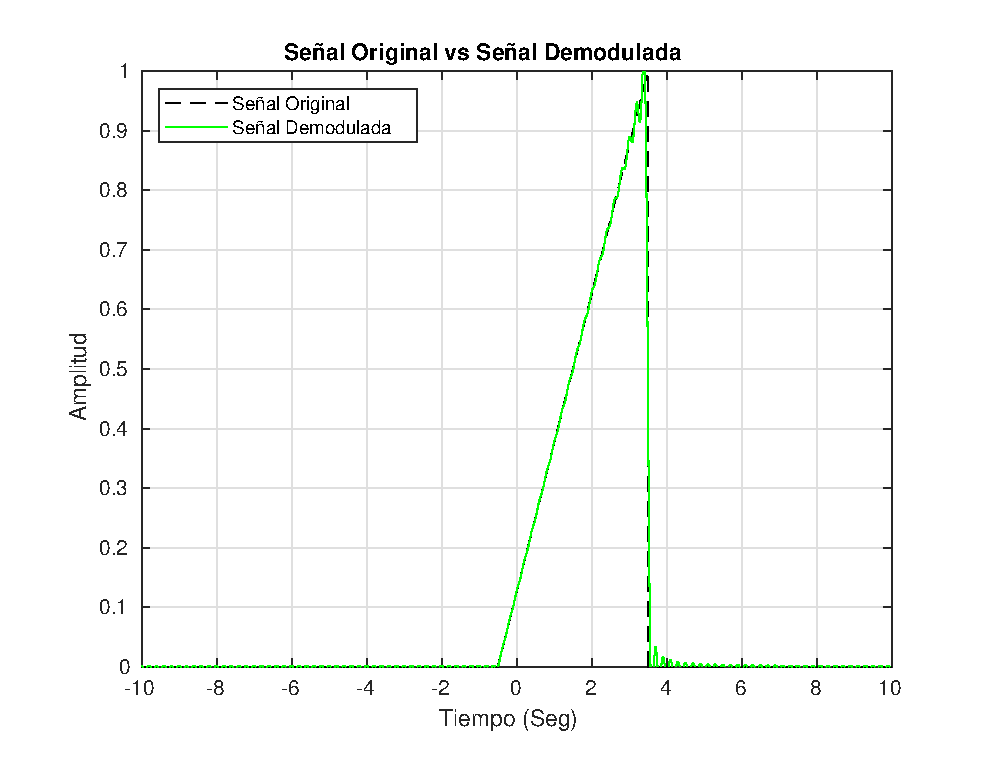
\includegraphics[width=5.1cm]{img/Comp_Tim/Comp_Tim.eps}
		\caption{\scriptsize Error de fase de 60 grados.}
		\label{subfig:inoutTiempo}
	\end{subfigure}
	\begin{subfigure}[b]{0.495\linewidth}
		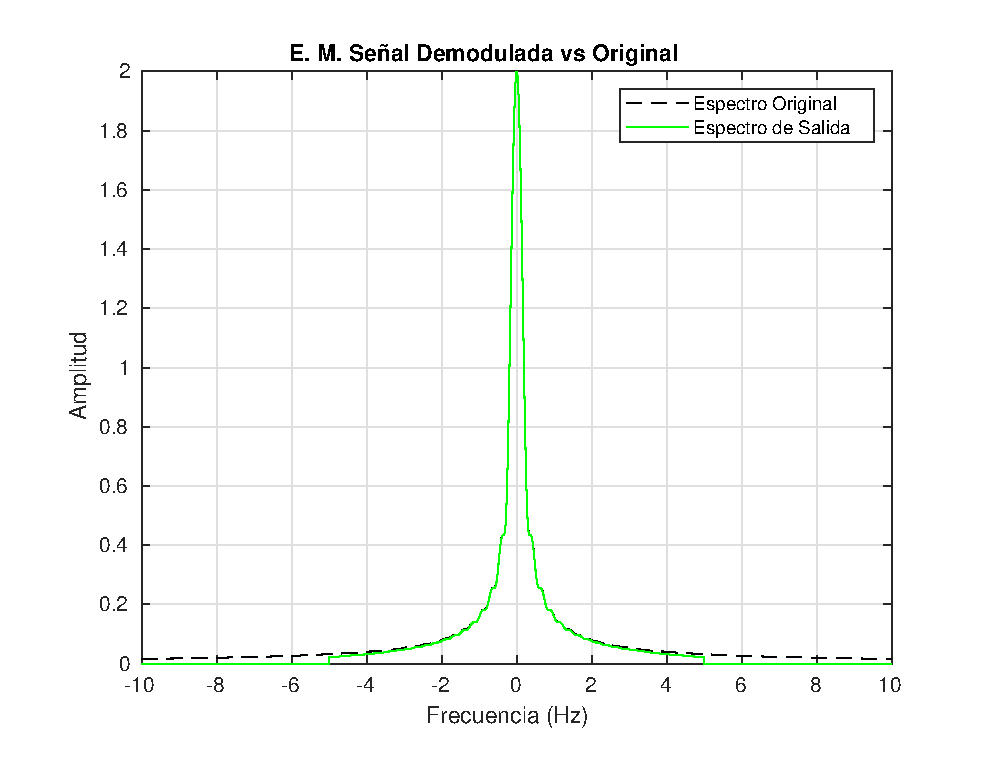
\includegraphics[width=5.1cm]{img/Comp_EM/Comp_EM.eps}
		\caption{\scriptsize Sin error de fase.}
		\label{subfig:inoutFrecuencia0}
	\end{subfigure}
	\vspace{-3mm}
	\caption{\scriptsize Señales de salida con errores de sincronismo en fase.}
	\label{fig:inoutSistema}
	\vspace{-5mm}
\end{figure}

\subsection{Desarrollo del objetivo clave 1-Análisis de resultados sin introducir errores de sincronismo}

\subsection{Desarrollo del objetivo clave 2-Introducir errores de sincronismo en fase}

Para el escenario planteado de falta de sincronismo de fase, se realizaron iteraciones de la simulación variando el valor de sincronismo de fase en pasos de 45 grados.
Se hace uso de los valores de Energía y MSE para tener una aproximación cuantitativa de la modificación que sufre la señal de salida con respecto a la señal de entrada.

\begin{figure}[H]
	\centering
	\begin{subfigure}[b]{0.49\linewidth}
		\def\svgwidth{5cm}
		\input{img/DFase0/DFase0.pdf_tex}
		\caption{\scriptsize Sin error de fase.}
		\label{subfig:DFase0}
	\end{subfigure}
	\begin{subfigure}[b]{0.49\linewidth}
		\def\svgwidth{5cm}
		\input{img/DFase60/DFase60.pdf_tex}
		\caption{\scriptsize Error de fase de 60 grados.}
		\label{subfig:DFase60}
	\end{subfigure}
	\begin{subfigure}[b]{0.49\linewidth}
		\def\svgwidth{5cm}
		\input{img/DFase90/DFase90.pdf_tex}
		\caption{\scriptsize Error de fase de 90 grados.}
		\label{subfig:DFase90}
	\end{subfigure}
	\begin{subfigure}[b]{0.49\linewidth}
		\def\svgwidth{5cm}
		\input{img/DFase180/DFase180.pdf_tex}
		\caption{\scriptsize Error de fase de 180 grados.}
		\label{subfig:DFase180}
	\end{subfigure}
	\vspace{-3mm}
	\caption{\scriptsize Señales de salida con errores de sincronismo en fase.}
	\label{fig:graficasfase}
	\vspace{-5mm}
\end{figure}

Es evidente que el sincronismo de fase introduce atenuación lineal en el rango de 0 a 90 grados (figuras \ref{subfig:DFase0}, \ref{subfig:DFase60}, \ref{subfig:DFase90}). Sin embargo, es interesante apreciar que, en el siguiente rango de frecuencias, esta atenuación se revierte con el signo contrario. Por lo que la MSE alcanza su valor máximo de error en 180 grados (figura \ref{fig:erroresFase}), que es cuando la señal es mas similar a la señal de entrada, pero multiplicada por -1 (figura \ref{subfig:DFase180}).
\begin{table}[H]
	\centering
	\caption{\scriptsize}
	\label{tab:varacionFrecuencia}
	\vspace{-3mm}
	\tiny\begin{tabular}{|l|c|c|c|c|c|}
		\hline
		Variación Fase         & 0       & 45      & 90      & 135            & 180   \\ \hline
		MSE Input-Output       & 0.00064  & 0.02940 & 0.33310    & 0.96830    & 1.32860 \\ \hline
		Energía Salida $A_c=2$ & 1.32800 & 0.66  & 0.0001 & 0.66360           & 1.32860 \\ \hline
		Energía Entrada        & 1.3332  & 1.3332  & 1.3332  & 1.3332         & 1.3332 \\ \hline \hline
		Variación Fase   & 180     & 225     & 270     & 315      & 360   \\ \hline
		MSE Input-Output       & 1.32860 & 0.96870 & 0.33350 & 0.02950   & 0.00064 \\ \hline
		Energía Salida $A_c=2$ & 1.32860 & 0.66440 & 0.00001 & 0.66360   & 1.32800 \\ \hline
		Energía Entrada        & 1.3332  & 1.3332  & 1.3332  & 1.3332   & 1.3332 \\ \hline
	\end{tabular}

\end{table}

% \begin{table}[H]
% 	\centering
% 	\caption{\scriptsize}
% 	\label{tab:variacionFrecuencia2}
% 	\vspace{-3mm}
% 	\tiny\begin{tabular}{|l|c|c|c|}
% 		\hline
% 		{Variación Frecuencia} & {MSE Input-Output} & {Energía Salida $A_c=2$} & {Energía Entrada} \\ \hline
% 		{-10}                  & 0.3988             & 0.3265                   & 1.332             \\ \hline
% 		{-1}                   & 0.50210            & 0.6629                   & 1.332             \\ \hline
% 		{-0.5}                 & 0.65               & 0.6603                   & 1.332             \\ \hline
% 		{-0.1}                 & 0.40410            & 0.2493                   & 1.332             \\ \hline
% 		{-0.01}                & 0.00076            & 1.2924                   & 1.332             \\ \hline
% 		{0}                    & 0.00064            & 1.328                    & 1.332             \\ \hline
% 		{0.01}                 & 0.00074            & 1.2927                   & 1.332             \\ \hline
% 		{0.1}                  & 0.40370            & 0.2486                   & 1.332             \\ \hline
% 		{0.5}                  & 0.65770            & 0.6604                   & 1.332             \\ \hline
% 		{1}                    & 0.50210            & 0.6629                   & 1.332             \\ \hline
% 		{10}                   & 0.39880            & 0.3265                   & 1.332             \\ \hline
% 	\end{tabular}
% \end{table}

Los valores máximos de energía se tienen en 0 y 180 grados, sin embargo, en estos mismos puntos se tienen los valores mínimo y máximo de energía de la señal. Esto nos permite concluir que la energía por si sola, no es un referente ideal para medir la integridad o la perdida de información de una señal que ha atravesado un sistema.
\begin{figure}[H]
	\centering
	\def\svgwidth{8.8cm}
	\tiny\input{img/ErroresFase/ErroresFase.pdf_tex}
	\caption{\scriptsize Variación de fase contra MSE y energía.}
	\vspace{-3mm}
	\label{fig:erroresFase}
\end{figure}
Al ser la señal evaluada una señal no periódica con espectro de frecuencia infinito centrado en banda base, cualquier filtrado pasa bajo introduce distorsión lineal, sin embargo, si no se tiene en cuenta la distorsión generada por el filtro, se puede afirmar que la modificación de la señal producida por el de-sincronismo de fase no califica como distorsión lineal ya que aparentemente afecta a todas las componentes de frecuencia dentro del rango del modulador de una manera similar.

\subsection{Desarrollo del objetivo clave 3-Introducir errores de sincronismo en frecuencia}
Para este escenario se realizaron iteraciones de la simulación variando el valor de sincronismo en frecuencia para los valores observados en la tabla. Se realizó de esta manera ya que a diferencia de como ocurría en los errores de fase, en los errores de frecuencia no se observa una relación lineal de ocurrencia y pequeños cambios en el sincronismo afectan de manera significativa a la señal, sobre todo, en valores cercanos a una variación de frecuencia igual a cero.
% \begin{table}[H]
% 	\centering
% 	\caption{\scriptsize }
% 	\label{tab:varacionFrecuencia}
% 	\vspace{-3mm}
% 	\tiny\begin{tabular}{|l|c|c|c|c|c|}
% 		\hline
% 		Variación Frecuencia   & -10     & -1      & -0.5    & -0.1    & -0.01   \\ \hline
% 		MSE Input-Output       & 0.3988  & 0.50210 & 0.65    & 0.40410 & 0.00076 \\ \hline
% 		Energía Salida $A_c=2$ & 0.3265  & 0.66290 & 0.66030 & 0.24930 & 1.29240 \\ \hline
% 		Energía Entrada        & 1.3332  & 1.3332  & 1.3332  & 1.3332  & 1.3332  \\ \hline \hline
% 		Variación Frecuencia   & 0.01    & 0.1     & 0.5     & 1       & 10      \\ \hline
% 		MSE Input-Output       & 0.00074 & 0.40370 & 0.65770 & 0.50210 & 0.39880 \\ \hline
% 		Energía Salida $A_c=2$ & 1.29270 & 0.24860 & 0.66040 & 0.66290 & 0.32650 \\ \hline
% 		Energía Entrada        & 1.3332  & 1.3332  & 1.3332  & 1.3332  & 1.3332  \\ \hline
% 	\end{tabular}
% 
% \end{table}

\begin{table}[H]
	\centering
	\caption{\scriptsize}
	\label{tab:variacionFrecuencia2}
	\vspace{-3mm}
	\tiny\begin{tabular}{|l|c|c|c|}
		\hline
		{Variación Frecuencia} & {MSE Input-Output} & {Energía Salida $A_c=2$} & {Energía Entrada} \\ \hline
		{-10}                  & 0.3988             & 0.3265                   & 1.332             \\ \hline
		{-1}                   & 0.50210            & 0.6629                   & 1.332             \\ \hline
		{-0.5}                 & 0.65               & 0.6603                   & 1.332             \\ \hline
		{-0.1}                 & 0.40410            & 0.2493                   & 1.332             \\ \hline
		{-0.01}                & 0.00076            & 1.2924                   & 1.332             \\ \hline
		{0}                    & 0.00064            & 1.328                    & 1.332             \\ \hline
		{0.01}                 & 0.00074            & 1.2927                   & 1.332             \\ \hline
		{0.1}                  & 0.40370            & 0.2486                   & 1.332             \\ \hline
		{0.5}                  & 0.65770            & 0.6604                   & 1.332             \\ \hline
		{1}                    & 0.50210            & 0.6629                   & 1.332             \\ \hline
		{10}                   & 0.39880            & 0.3265                   & 1.332             \\ \hline
	\end{tabular}
\end{table}

Es posible apreciar que para los valores cercanos a la frecuencia central (en este caso banda base), la distorsión y la energía sirven como indicadores de integridad de la señal. Siendo esto apreciable en la figura \ref{subfig:DFreq0} y \ref{subfig:DFreq001}.

\begin{figure}[H]
	\centering
	\begin{subfigure}[b]{0.49\linewidth}
		\def\svgwidth{5cm}
		\input{img/DFreq0/DFreq0.pdf_tex}
		\caption{\scriptsize En sincronismo.}
		\label{subfig:DFreq0}
	\end{subfigure}
	\begin{subfigure}[b]{0.49\linewidth}
		\def\svgwidth{5cm}
		\input{img/DFreq001/DFreq001.pdf_tex}
		\caption{\scriptsize Error de 0.01 Hz.}
		\label{subfig:DFreq001}
	\end{subfigure}
	\begin{subfigure}[b]{0.49\linewidth}
		\def\svgwidth{5cm}
		\input{img/DFreq01/DFreq01.pdf_tex}
		\caption{\scriptsize Error de 0.1 Hz.}
		\label{subfig:DFreq01}
	\end{subfigure}
	\begin{subfigure}[b]{0.49\linewidth}
		\def\svgwidth{5cm}
		\input{img/DFreq1/DFreq1.pdf_tex}
		\caption{\scriptsize Error de 1 Hz.}
		\label{subfig:DFreq1}
	\end{subfigure}
	\vspace{-3mm}
	\caption{\scriptsize Señales de salida con errores de sincronismo en frecuencia.}
	\label{fig:graficasfreq}
	\vspace{-5mm}
\end{figure}

En valores de cambio de frecuencia superiores a los mencionados, la señal es reemplazada por un trozo de onda senoidal de frecuencia directamente proporcional al de-sincronismo en frecuencia aplicado. La señal original aparece como envolvente de esta onda. Este comportamiento se presenta hasta que el de-sincronismo es mayor al ancho de banda del filtro pasa bajo. Esto debido a que la componente de frecuencia de la señal original deformada por la falta de sincronismo en frecuencia es absorbida por este filtro.
\begin{figure}[H]
	\centering
	\def\svgwidth{8.8cm}
	\tiny\input{img/ErroresFrecuencia/ErroresFrecuencia.pdf_tex}
	\caption{\scriptsize Variación de frecuencia contra MSE y energía.}
	\vspace{-3mm}
	\label{fig:erroresFreucencia}
\end{figure}
Esta tendencia se observa en la figura \ref{fig:erroresFreucencia}, donde se aprecia que en los extremos, la energía cae, y el error medio cuadrático comienza a estabilizarse a valores cercanos a 0.33, los cuales se dan cuando la señal no está presente (tal como se aprecia en el caso de desfase a 90 grados).


\subsection{Desarrollo del objetivo clave 4-Introducir ambos tipos de errores de sincronismo.}


\begin{figure}[H]
	\centering
	\begin{subfigure}[b]{0.49\linewidth}
		\def\svgwidth{5cm}
		\input{img/EMF90_freq0/EMF90_freq0.pdf_tex}
		\caption{\scriptsize En sincronismo.}
		\label{subfig:EMF90_freq0}
	\end{subfigure}
	\begin{subfigure}[b]{0.49\linewidth}
		\def\svgwidth{5cm}
		\input{img/EMF90_freq001/EMF90_freq001.pdf_tex}
		\caption{\scriptsize Error de 0.01 Hz.}
		\label{subfig:EMF90_freq001}
	\end{subfigure}
	\begin{subfigure}[b]{0.49\linewidth}
		\def\svgwidth{5cm}
		\input{img/EMF90_freq01/EMF90_freq01.pdf_tex}
		\caption{\scriptsize Error de 0.1 Hz.}
		\label{subfig:EMF90_freq01}
	\end{subfigure}
	\begin{subfigure}[b]{0.49\linewidth}
		\def\svgwidth{5cm}
		\input{img/EMF90_freq1/EMF90_freq1.pdf_tex}
		\caption{\scriptsize Error de 1 Hz.}
		\label{subfig:EMF90_freq1}
	\end{subfigure}
	\vspace{-3mm}
	\caption{\scriptsize Señales de salida con errores de sincronismo en fase de $90^\circ$ y variación en frecuencia.}
	\label{fig:graficasFase90freq}
	\vspace{-5mm}
\end{figure}

\section{Conclusiones}%
\label{sec:conclusiones}
\begin{itemize}
    \item El sincronismo de fase es necesario para mantener la estabilidad espectral de la modulación en la región de banda base
    \item El filtrado pasa bajas en la demodulación nos permite recuperar la señal en banda base, sin embargo, la frecuencia de modulación debe ser lo suficientemente grande para que las componentes espectrales de la modulación no entren en el rango del ancho de banda del filtro
    \item Cuando se tiene de-sincronismo cruzado de fase y frecuencia, la componente de banda base de la señal vuelve a aparecer súbitamente (teniendo valores de desfase de 90 grados) aun con pequeñas variaciones en la frecuencia del demodulador.
    \item En el de sincronismo de fase, las componentes de frecuencia cercanas a banda base disminuyen proporcionalmente en el rango de 0 a 90 grados, a partir de este valor, vuelve a incrementar, sin embargo, la señal ahora tiene una polaridad invertida.
    \item Como la señal no es periódica (y toda su información está en banda base) métodos de análisis de distorsión como la distorsión armónica total no son aplicables.
    \item El umbral a partir del cual la distorsión de la señal aumenta de forma drástica es independiente de la frecuencia de modulación (siempre y cuando esta frecuencia supere el ancho de banda del filtro pasa bajo del receptor) y depende del periodo de la señal.
    \item El de sincronismo de frecuencia es similar a tener múltiples de sincronismos de fase variando a lo largo de distintos instantes de tiempo. Es por esto por lo que la señal demodulada es muy sensible a los cambios de frecuencia. Sin embargo, se puede evidenciar en las gráficas que es posible recuperar la señal original, ya que la misma aparece como envolvente de una onda senoidal de frecuencia equivalente al de sincronismo en frecuencia.
    \item El rango de sincronismo en frecuencia en el cual sería posible recuperar la señal a partir de la envolvente de la señal demodulada, sería igual al ancho de banda del filtro pasa bajos del receptor, ya que, si el de sincronismo es más grande, la información contenida en el espectro "desfasado en frecuencia" simplemente seria eliminada por este filtro.
    \item Para el caso del de sincronismo de fase, un rectificador de onda completa se propondría como una posible solución para recuperar la onda atenuada por el desfase de la onda demoduladora.
\end{itemize}

\input{codigofuente/apendice}
\printbibliography[title={Bibliografía}]
\end{document}
%---------------------------------------------
